\documentclass{article}%
\usepackage{graphicx}
\usepackage[T1]{fontenc}%
\usepackage[utf8]{inputenc}%
\usepackage{lmodern}%
\usepackage{textcomp}%
\usepackage{lastpage}%
\usepackage[export]{adjustbox}
\usepackage[top=1in, bottom=1.25in, left=1.00in, right=1.00in]{geometry}
%
\title{A Summary of Don't Make Me Think}%
\author{Hal DiMarchi}%
%
\begin{document}%
\normalsize%
\begin{titlepage}
  \pagenumbering{gobble}
  \centering
  \vfill
  {\bfseries\Large
      A Summary of Don't Make Me Think\\
      H. DiMarchi\\
  }
  \vfill
  \begin{figure}[h]
    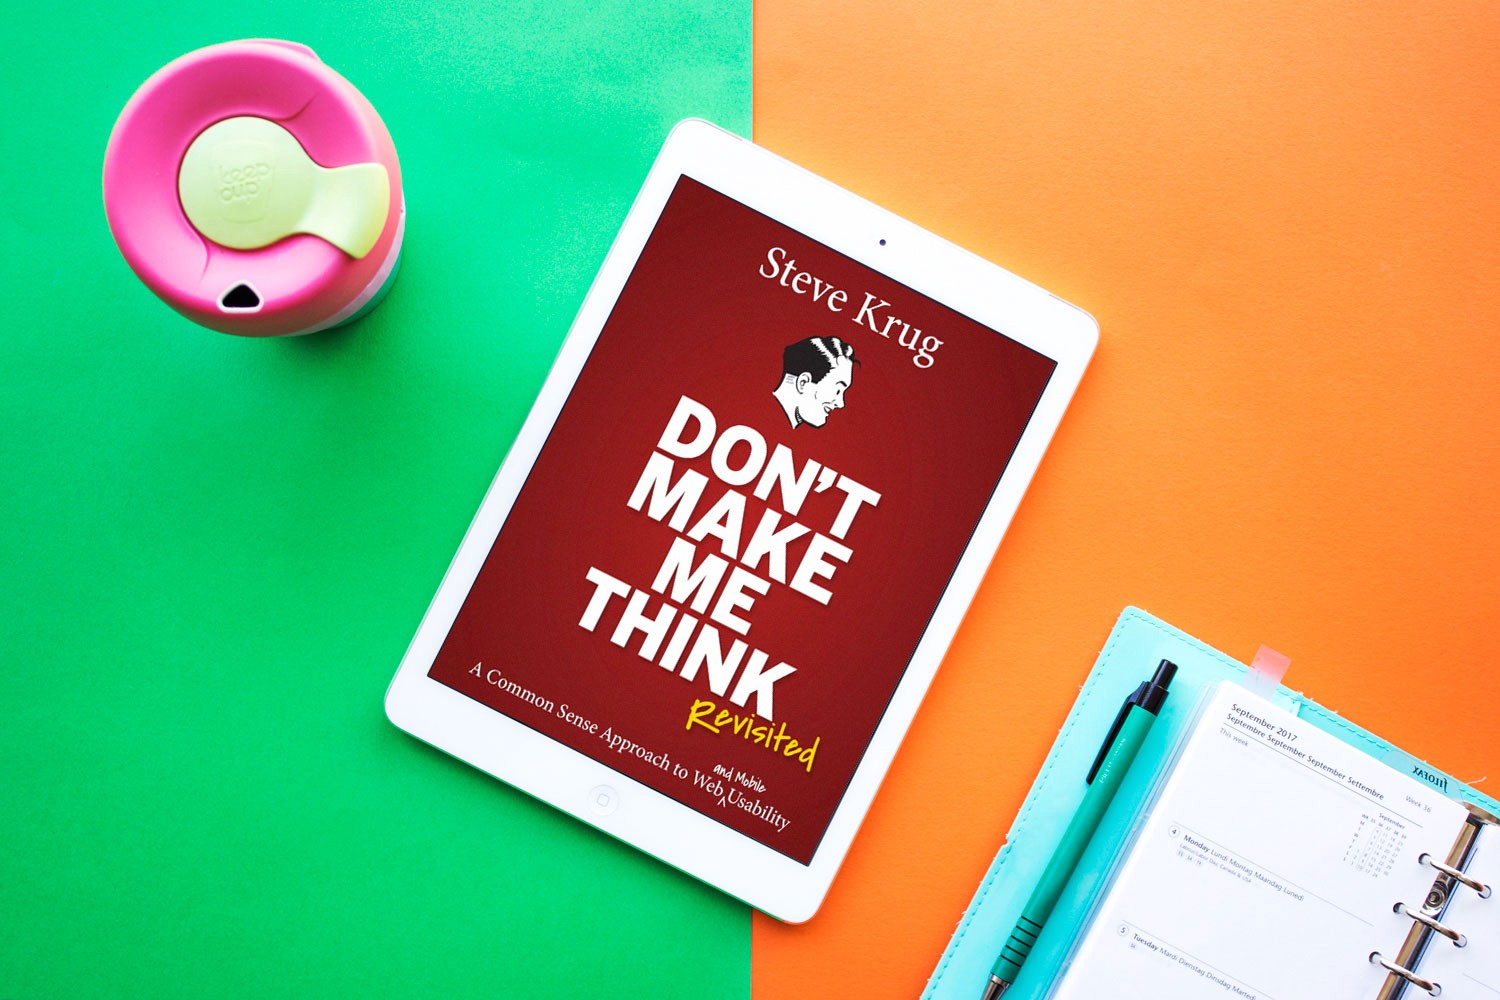
\includegraphics[width=1.32\textwidth, center]{nothinkyitsstinky}
  \end{figure}
  \vfill
\end{titlepage}
\pagenumbering{gobble}%
\newpage%
\tableofcontents%
\newpage%
\section{Introduction}%
\label{sec:Introduction}%
  Don't Make Me Think outlines Krugs idea of good website and webpage design. Many of
  the ideas he presents extend to other products and their design.
  Krug begins his book with a few things that aren't central to the core material.
  This excludes his definition of usability.
  \subsection{Usability}
    In Krugs words, a product is \textbf{usable} if: \newline
    ``A person of average (or even below average) ability and experience can figure out how to
    use the thing to accomplish something without it being more trouble than it’s worth.''
    \newline
    In other words if a users desire to use the thing is stronger than the users desire
    to not have to learn something or figure it out, the product is usable. It is more
    difficult to make a thing usable when the user isn't heavily invested in its use.



%
\section{Guiding Principles}%
\label{sec:Guiding Principles}%
\subsection{Don't Make Me Think}
I'll say it again; \textbf{Don't Make Me Think}.
  \subsubsection{The First Law of Usability}
  The sentiment, don't make me think, is Krugs first law of usability.
  It refers to the idea that an interface should not make the user ask questions
  about the interface and have to navigate it. Their thoughts should have periods.
  Not question marks. If this can be accomplished we can describe the interface, and how to use it,
  as \textbf{self-evident}. \newline

  Sometimes this cannot be accomplished and so we have to settle for making an
  interface \textbf{self-explanatory}. This means a little, nearly effortless, thought
  is involved in understanding the interface.
  \newline

  These are some important questions a user should not have to ask about an interface:
  \begin{itemize}
    \item Where am I?
    \item Where should I begin?
    \item Where did they put $\rule{1cm}{0.15mm}$ ?
    \item What are the most important things on this page?
    \item Why did they call it that?
    \item Is that an ad or part of the site?
  \end{itemize}

\subsection{How We Really Use the Web}
This chapter is summarized by ``Three Facts of Life''.
  \subsubsection{Fact 1: We Don't Read Pages, We Scan Them}
    We\slash users will not read an entire webpage and then make a decision
    about what to do next. We scan the page for particular words, phrases, or
    other cues to identify what they are looking for. \newline
    We do this for three reasons:
    \begin{enumerate}
      \item ``We're usualy on a mission''
      \item ``We know we don't \emph{need} to read everything''
      \item ``We're good at it''
    \end{enumerate}
  \subsubsection{Fact 2: We Don't Make Optimal Choices. We Satisfice.}
    We choose the first reasonable option (satisficing), not the best one. \newline
    According to Krug we do this for four reasons:
    \begin{enumerate}
      \item ``We're usually in a hurry''
      \item Not much of a cost for guessing wrong
      \item ``Weighing options might not improve our chances''
      \item ``Guessing is more fun''
    \end{enumerate}
  \subsubsection{Fact 3: We Don't Figure Out How Things Work, We Muddle Through.}
    In other words we don't go out of our way to come to an accurate understanding
    about how the thing we're using works. We rely on instincts, associations, and
    limited reasonings without any broader comprehension of what we're doing.\newline
    We do this for two reasons:
    \begin{enumerate}
      \item It's not important to us, we just want to use the thing
      \item ``If we find something that works, we stick with it''
    \end{enumerate}
    This makes it all the more important for interfaces to be designed well. If a user
    can effortlessly comprehend the thing they are using they will avoid inefficiencies
    and errors, leading to a better experience. But if comprehension isn't effortless
    they won't bother.
\subsection{Designing Great Billboards}
  Knowing how users behave we have to use techniques that will maximize their
  absorption of information they could, or must, use. \newline
  Krug offers up 6 techniques and conventions:
  \begin{enumerate}
    \item Conventions are your friends; users will respond better to things that are familiar to them
    \item Create effective visual hierarchies
    \item Break pages up into clearly defined areas
    \item Make it obvious what is clickable
    \item Keep the \emph{noise} down to a dull roar. \emph{Noise} refers to
      \begin{itemize}
        \item Shouting: when everything on a page is loud and clammoring for your attention.
        \item Disorganization: Why is this here and that there?
        \item Clutter: If there's too much assume everything is visual clutter until proven otherwise.
      \end{itemize}
    \item Format text to support scanning
  \end{enumerate}
  \subsubsection{Needless Words}
  An effective way of reducing visual noise is to get rid of needless words.
  Words that are needless can add fluff to a sentence or concern something nobody cares
  enough to readabout. \newline
  A special case of needless words is \textbf{Happy Talk}. Happy Talk is something like:\newline
  ``Hello and welcome to my website, I am very happy you are here!!!''. Happy talk must be removed.
  It doesn't do anything except annoy and incovenience users. Happy talk will actually make people less happy.
%
\section{Things You Need to Get Right}%
\label{sec:Things You Need to Get Right}%
  \subsection{Web Navigation}
    \paragraph{Purpose of Navigation}
    Navigation exists to:
    \begin{itemize}
      \item Help us find what we're looking for.
      \item Tell us where we are.
      \item Tell us what is here.
      \item Give us confidence in the people behind the site.
    \end{itemize}
  \subsubsection{Key Navigation Elements}
    It is important to note that websites should be organized along some sort of hierarchy
    that is relevant to the contents of the website. This hierarchy is used for browsing
    a website. A user may also search, usually by text, across a website. This relies less
    on this hierarchy.
    \paragraph{Global Navigation:}
      Global Navigation is the set of navigation elements that appear on every
      page of a website. It is composed of four elements:
      \begin{enumerate}
        \item Site ID: The name of the site. Tells us what website we are on. This is the top of our hierarchy.
        \item Utilities: Things that can help us use the site, such as an option to sign in, or contact the company.
        \item Sections: Sections in the global navigation represent the primary level of the site hierarchy.
        \item Search: This is where a user can go to search for something. Because it is in the global navigation a user
                      can always jump to it if they have given up on browsing. In my mind this turns a potential
                      abandoment of the site into a search process.
      \end{enumerate}
    \paragraph{Home Page Button:}
      The Site ID, or one of the sections, should link to the home page of a website.
      This gives users confidence because they can always start over.
    \paragraph{Page Names:}
      Page names are IDs for each and \emph{every} webpage on a website. \newline
      Page names should:
      \begin{itemize}
        \item Appear to be framing the content that is unique to their page
        \item Be prominent.
        \item Match what was clicked. The button text should match the page name.
      \end{itemize}
    \paragraph{You Are Here:}
      Navigation elements can often be modified to give us an idea of where we are
      on a website. For instance we can highlight the navigation element we clicked
      on to go to the page we are on. This allows us to see where we are in the
      hierarchy of the website.
    \paragraph{Breadcrumbs:}
      This is a breadcrumb: Home > A category > A subcategory > \textbf{Where we are now}
      \newline Breadcrumbs should be:
      \begin{itemize}
        \item At the top of the page.
        \item Use > between levels.
        \item Have the last item bolded.
      \end{itemize}
      These tell us where we are and how we got there.
  \subsubsection{Trunk Test}
    The questions of the Trunk Test are:
    \begin{itemize}
      \item What site am I on? (Site ID)
      \item What page am I on? (Page Name)
      \item What are the major sections of this site? (Sections)
      \item What are my options at this level? (Local navigation)
      \item Where am I in the scheme of things? (``You are here'' indicators.)
      \item How can I search? (Search)
    \end{itemize}
    Each page on your website should answer these questions.


%
\section{Making Sure You Got Them Right}%
\label{sec:Making Sure You Got Them Right}%
  Often websites are designed by teams. Often these teams
  disagree.
  \subsection{Common Disagreements}
    \paragraph{Everybody Likes:}
      Some team members will assert that everybody likes or doesn't like some
      navigation element or style, usually because they do. They are always wrong.
      The important lesson is that we tend to think users are like us, and that we
      have to check that instinct at the door.
    \paragraph{Farmers vs. Cowmen:}
      Everyone involved in designing a website or other tool will have a different
      perspective on what the user experience of it should be based on the professional
      goals they have and the kind of work they do.
    \paragraph{The Myth of the Average User:}
      There is no average user. All users are unique, as is their use of the web.
  \subsubsection{The Antidote for Religious Debates}
    People tend to debate over large questions like, ``Do people like check boxes?''.
    These questions are not important. It is more important to ask if \emph{that} check box
    on \emph{this} page creates the experience we want for most people who are likely to use
    \empha{this} site. Usually the \textbf{debate is best replaced by usuability testing}. Watch
    people use it instead of talking about them using it.
  \subsection{Usability Testing}
    ``\textbf{Usability Tests} are about watching one person at a time try to use something (whether it’s aWeb site, a prototype, or some sketches of a new design) to do typical tasks so you can detect
and fix the things that confuse or frustrate them.''
    \subsubsection{Several Truths about Usability Testing}
    \begin{enumerate}
      \item ``If you want a great site, you've got to test.''
      \item ``Testing one user is 100 percent better than testing none.''
      \item ``Testing one user early in the project is better than testing 50 near the end.''
    \end{enumerate}
    \subsubsection{Who, What, When, Where, How}
    Krug outlines an ideal usability testing process for a webpage. This is somewhat
    flexible to specific project requirements.
    \begin{itemize}
      \item \textbf{Who}: Three loosely recruited ``Users''. They do not have to be exactly like your target audience.
      \item \textbf{What}: Watch someone use your site and identify the most serious problems they run into.
      \item \textbf{When}: One morning a month, the same day each month.
      \item \textbf{Where}: On-site with observers in a conference room using screen sharing to view the users.
      \item \textbf{How}: The entire team debriefs over lunch the same day to compare notes and decide what to fix. This results in a short 1 to 2 page report.
    \end{itemize}
    \subsubsection{Debriefing}
    After your usability testing you will gather with your team over lunch to identify
    serious problems. It is extremely important to focus on identifying and fixing
    the most serious problems in the order of seriousness. \newline Krug gives us some steps
    to follow:
    \begin{enumerate}
      \item Make a collective list.
      \item Choose the ten most serious problems.
      \item Rate them on a 1 to 10 scale.
      \item Create an ordered list - now you're done!
    \end{enumerate}
    Some other tips for making this happen:
    \begin{itemize}
      \item Keep a separate list of problems that aren't serious but take less than an hour to fix by \emph{one} person.
      \item Resist the impulse to add things to your page or site to fix the problem.
      \item Take new feature requests by the users with a grain of salt.
      \item Ignore problems that the user recovers from very quickly from without any prompting.
    \end{itemize}
\end{document}
